
\documentclass[tikz]{standalone}
\usepackage{tikz}
\usetikzlibrary{calc}

\usepackage{units}

\newcommand*{\Margin}{0.9}%
\newcommand*{\Distance}{4.5}%


\begin{document}
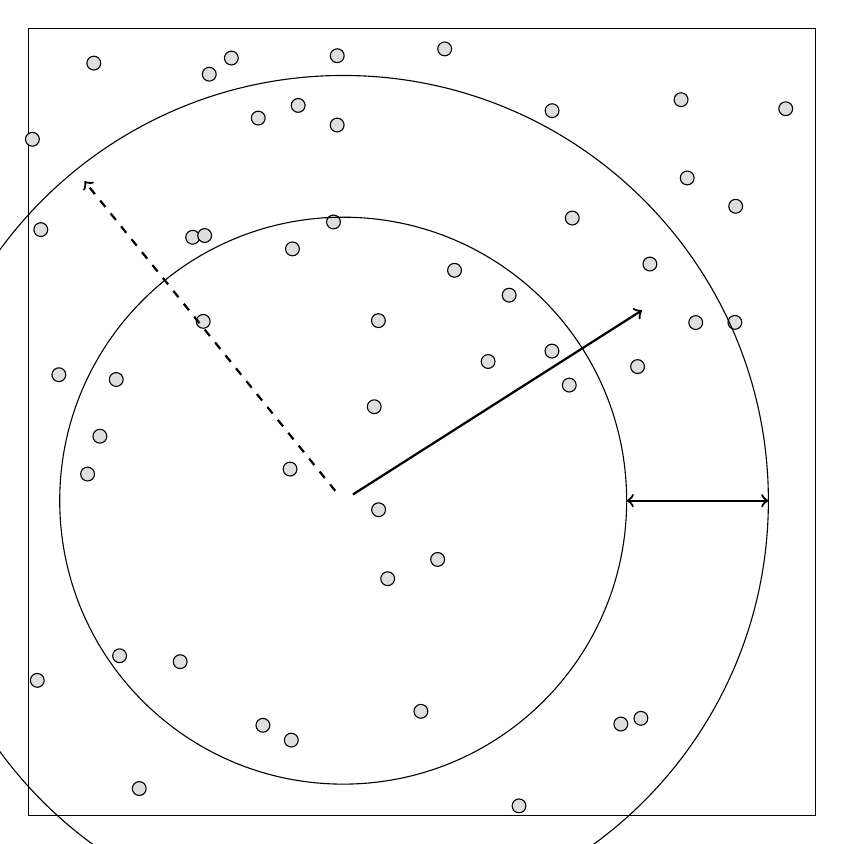
\begin{tikzpicture}

  \draw[use as bounding box] (0,0) rectangle (10,10);

  \foreach \i in {1,2,...,50}{
    \pgfmathsetmacro{\x}{rnd*10.}
    \pgfmathsetmacro{\y}{rnd*10.}

    \node[draw, circle, inner sep=0, minimum size=5., fill=gray!25] at (\x,\y) {};
    }

  \node (Origin) at (4,4) {};

  \draw (Origin) circle (\Distance+\Margin);
  \draw (Origin) circle (\Distance-\Margin);
    %++ is relative to Origin!
  \draw[thick, ->] (Origin) -- ++(32.5:\Distance);

  \draw[thick, <->] ($(Origin)+(\Distance-\Margin,0)$) -- ($(Origin)+(\Distance+\Margin,0)$);

  \draw[thick, dashed, ->] (Origin) -- ++(129:\Distance+\Margin*0.8);

\end{tikzpicture}
\end{document}
%%% Local Variables: 
%%% mode: latex
%%% TeX-master: t
%%% End: 
